% -*- mode: latex -*-

\mansection{cartesian to spherical coordinates transformations}
\begin{mandesc}
   \short{cart2sph}{cartesian to spherical coordinates}\\
   \short{sph2cart}{spherical to cartesian coordinates}
\end{mandesc}

%-- Calling sequence section
\begin{calling_sequence}
\begin{verbatim}
 [theta, phi, r] = cart2sph(x, y, z)
 [theta, phi, r] = cart2sph(x, y, z, colat=%t)
 [x, y, z] = sph2cart(theta, phi, r)
 [x, y, z] = sph2cart(theta, phi, r, colat=%t)
\end{verbatim}
\end{calling_sequence}

%-- Parameters
\begin{parameters}
  \begin{varlist}
   \vname{x, y, z}: real vectors or matrices of same dimensions
   \vname{colat}: boolean optional named argument (default is \%f)
   \vname{theta, phi, r}: real vectors or matrices
  \end{varlist}
\end{parameters}

\begin{mandescription}
  Computes correspondance between cartesian coordinates $(x,y,z)$ and spherical
  coordinates $(\theta,\phi,r)$ :
\begin{itemize}
\item $\theta$ the azimuth angle (in $[0,2\pi)$)
\item $\phi$ the latitude (or elevation) angle by default or
      when \verb+colat=%f+ (here $\phi$ is in $[-pi/2,pi/2]$) or 
      the colatitude angle when \verb+colat=%t+ (in this case  $\phi$ is in $[0,pi]$)
\item and $r$ the euclidian distance between $O=(0,0,0)$ and $M=(x,y,z)$.
\end{itemize}

$$
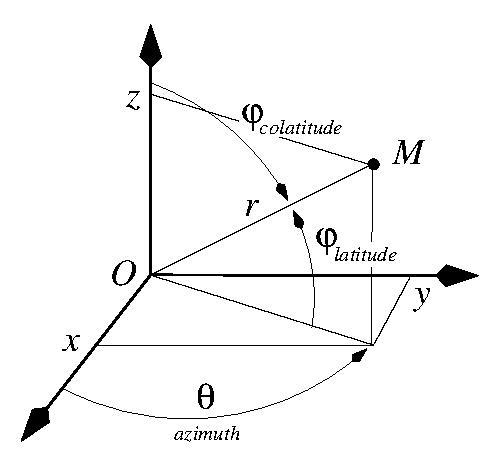
\includegraphics[width=8cm]{spherical} 
$$

We have the relations:
$$
\mbox{with } \varphi \mbox{ latitude}: 
\left\{\begin{array}{l}
x = r \cos(\theta) \cos(\varphi) \\
y = r \sin(\theta) \cos(\varphi) \\
z = r \sin(\varphi)
\end{array}\right.
\mbox{                  and with } \varphi \mbox{ colatitude}: 
\left\{ \begin{array}{l}
x = r \cos(\theta) \sin(\varphi) \\
y = r \sin(\theta) \sin(\varphi) \\
z = r \cos(\varphi)
\end{array} \right.
$$


\paragraph{remark}
One or two input argument(s) could be a scalar.
  
\end{mandescription}

%--example 
\begin{examples}
\begin{program}\HCode{[theta,phi,r]=cart2sph(1,1,sqrt(2))\Hnewline
// theta and phi must be equal to pi/4 and r must be equal to 2\Hnewline
[x,y,z] = sph2cart(theta, phi, r)\Hnewline
// x, y and z should be equal or very near 1, 1 and sqrt(2)}
\end{program}
\end{examples}


